\documentclass{neu_handout}
\usepackage{url}
\usepackage{amssymb}
\usepackage{amsmath}
\usepackage{marvosym}
\usepackage{graphicx}
\usepackage[pdftex]{graphicx}
\usepackage{subfigure}
\graphicspath{ {images/} }
\everymath{\displaystyle}

% Professor/Course information
\title{Homework 1 - Part 3}
\author{Emily Dutile}
\date{January 2018}
\course{CS7295}{Info Viz}

\begin{document}


\section*{Who is CS7295}

\subsection*{2. Data Type}

City - categorical \\
Country - categorical \\ 
State - categorical \\
Native language - categorical \\
Languages known other than English - categorical \\
Preferred OS - categorical \\
Mobile OS - categorical \\
Favorite language - categorical \\
Chocolate or Vanilla - categorical \\
Preferred OS - categorical \\
Color - categorical \\
Favorite number - categorical \\
Temperate - quantitative \\
Amount of coffee - quantitative \\
Wake up - quantitative \\
To bed - quantitative \\
Visual encoding - quantitative

\subsection*{4. Data Clean-Up}
To clean up the data, the data was exported to a new excel spreadsheet. Categorical data such as the Country which varied in naming convention (i.e.: USA vs United States) was manually corrected to be one category. In the category "what other languages do you speak besides English", I filled in blank values with None and also made multi-lingual students have comma separated values for languages. State abbreviations were spelled out as well or no values were changes to 'NA'. Some preprocessing was done around lengthy answers related to Mobile OS preference and removing words such as 'degrees'. Exclamation points were removed, numbers that were spelled out were many quantitative, and any temperature listed in something other than Fahrenheit was converted.

\subsection*{6. Data Gathering}
From Piazza I compared the information hints as to what text blurb matched with the data in the csv. I simply inserted two rows for department (CCIS or other) and what degree program the individual is pursuing. There wasn't a great deal of cleaning the data here.

\subsection*{7. Questions}

\subsubsection*{7.1}
Is there a correlation between bedtime and coffee consumption? Please see Appendices for visual.\\

There seems to be a high correlation between individuals that go to bed around 1am and the amount of coffee consumed. Overall, it appears that individuals who go to bed earlier at night seem to consume less coffee.

\subsubsection*{7.2}
Is there a typical “profile” for someone who prefers to use a mobile phone with an
Android versus Apple OS?

\subsection*{8. Additional Questions & Visualizations}


\subsubsection*{8.1}
Is there a correlation between preferred programming language and preferred OS? Please see Appendices for visual.\\

@TODO - justify your choice of visual encoding and visualization design choices (i.e., marks, channels,
perceptual ordering, etc.

\subsubsection*{8.2}
What percentage of the class speaks another language if their native language is not English? Please see Appendices for visual.\\

@TODO - justify your choice of visual encoding and visualization design choices (i.e., marks, channels,
perceptual ordering, etc.

\subsubsection*{8.3}
Are students sleeping enough? Please see Appendices for visual.\\

\appendix
\section{Appendices}

\subsection*{7.1}
\begin{figure}[h]
\centering
{
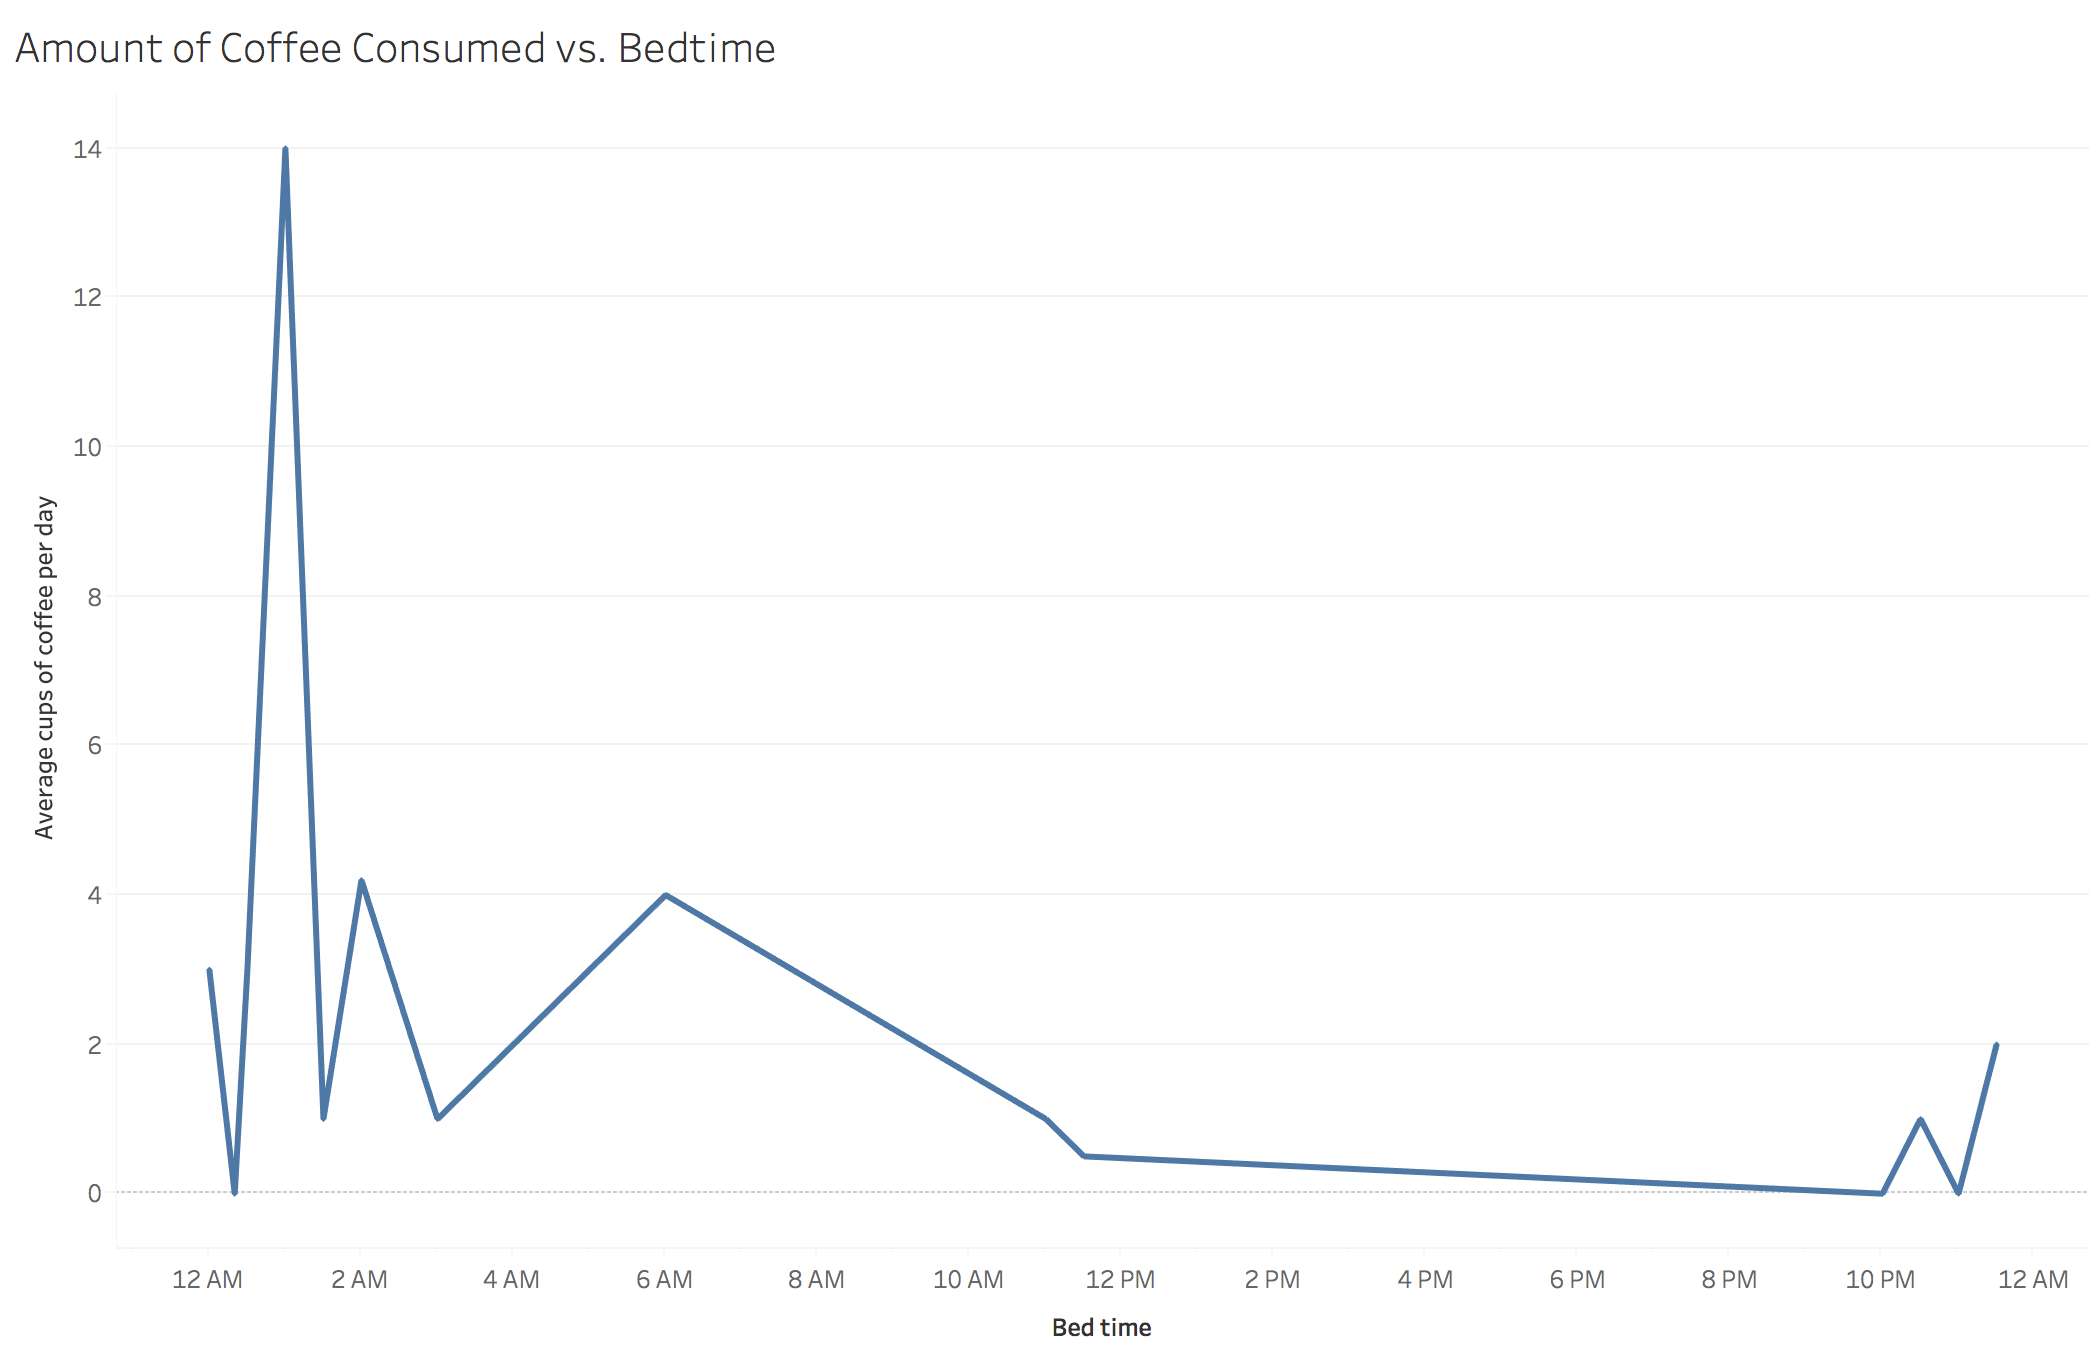
\includegraphics[width=0.7\linewidth]{bedtime_coffee}
}
\end{figure}


\end{document}
